\documentclass[12pt, a4paper]{article}
\usepackage{fancyhdr}
\usepackage[utf8]{inputenc}
\usepackage[english]{babel}
\usepackage[margin=2.5cm, left=1.5cm, right=1.5cm, top=2cm, bottom=2cm]{geometry}
\usepackage{amsmath, booktabs, enumitem, tikz, pgfplots, caption, titlesec}
\usepackage[colorlinks=true, linkcolor=black, citecolor=black, urlcolor=blue]{hyperref}
\usepackage{cleveref} % Erlaubt \cref{label}, das automatisch "Figure" oder "Table" schreibt
\pgfplotsset{compat=1.18}


\titleformat{\section}
    {\normalfont\large\bfseries}{\thesection}{1em}{}
\titleformat{\subsection}
    {\normalfont\normalsize\bfseries}{\thesubsection}{1em}{}
    
\setlength{\columnsep}{0.8cm}
\pagestyle{fancy}
\fancyhf{}
\rhead{\small Information \& Strategy}
\lhead{\small Voluntary Disclosure and Personalised Pricing}
\cfoot{\thepage}

\title{\normalsize \vspace{-3cm}\textbf{Voluntary Disclosure and Personalised Pricing: An Analysis of Tiered University Canteen Pricing}}
\author{\small Theo Osterhaus (Matriculation No. 7443693)}
\date{\vspace{-7ex}}

\begin{document}
\maketitle

\section{Introduction: The Value of Partial Disclosure}
As firms gain increasing access to consumer data, the economic debate has shifted from mere privacy concerns alone to the distribution of welfare. In their work, Ali, Lewis, and Vasserman (2022) explore whether consumers can increase their surplus by voluntarily providing evidence to a firm. This report applies their theoretical framework to a commonplace real-world example: the tiered pricing system of the \textit{Mensa}, a university canteen.
The \textit{Mensa} typically operates as a local monopolist for students and staff. It cannot force disclosure, and by requiring different forms of ID for access to specific price points, the system mirrors the 'rich Evidence' mechanism described in the paper. This report argues that consumers successfully avoid the 'punishing beliefs' of the monopolist by disclosing group membership (e.g. student status) rather than individual preferences. This strategic disclosure allows them to retain consumer surplus that would otherwise be lost under perfect price discrimination, ultimately resulting in measurable overall welfare gains.


\section{Case Study: Tiered Pricing as a Rich Evidence Mechanism}
The university canteen provides a compelling example of the rich evidence mechanism in a monopoly setting, with its four-tier pricing structure, summarised in \cref{tab:pricing_structure}:

\subsection{Empirical Validation and Revenue Benchmarking}
Empirical data from the \href{https://gb.kstw.de/2024/kennzahlen/}{Kölner Studierendenwerk (2024)} allows for a nuanced comparison. As detailed in \cref{tab:ksw_stats} 1.839 million meals were served and a total gastronomy revenue of EUR 11.28 million was generated. This gives an average revenue per meal of approximately EUR 6.13, strikingly close to the benchmark I created for my presentation of $p^*=6$. 
In our model, the weighted average of the four prices is EUR $7.75$, which naturally gravitates towards this mean, especially as students and staff (who are in the lower-priced tiers) typically account for the largest number of transactions.

\begin{table}[h]
    \centering
    \scriptsize
    
    \begin{minipage}{0.45\textwidth}
        \centering
        \captionof{table}{Empirical Snapshot KSW (2024)}
        \label{tab:ksw_stats}
        \begin{tabular}{@{}lr@{}}
            \toprule
            \textbf{Metric} & \textbf{Value (m. EUR)} \\ \midrule
            Meals Served & 1.839 m. units \\
            Gastronomy Revenue & 11.28 \\
            Personnel Costs & 26.17 \\
            Social Contributions & 16.21 \\
            State Grants & 5.35 \\ \midrule
            \textbf{Avg. Rev. / Meal} & \textbf{$\approx$ 6.13 EUR} \\ \bottomrule
        \end{tabular}
    \end{minipage}
    \hfill 
    \begin{minipage}{0.52\textwidth}
        \centering
        \captionof{table}{Rich Evidence vs. Benchmark Rent}
        \label{tab:pricing_structure}
        \begin{tabular}{@{}lccc@{}}
            \toprule
            \textbf{Group} & \textbf{Price} ($p_i$) & \textbf{Model} $CR_i$ & \textbf{Bench.} $CR$ \\ \midrule
            Students  & 3.30 EUR & \textbf{1.15} & 0.00 \\
            Staff     & 5.60 EUR & \textbf{0.70} & 0.00 \\
            Guests    & 7.00 EUR & \textbf{4.05} & 2.10 \\
            Externals & 15.10 EUR & \textbf{2.45} & 2.71 \\ \midrule
            \textbf{Total Avg.} & \textbf{7.75 EUR} & \textbf{2.09} & \textbf{4.81} \\ \bottomrule
        \end{tabular}
    \end{minipage}
    \vspace{0.5em}
\end{table}

However, the \textit{Mensa} example deviates from the model's assumption of a profit-maximising firm. The 2024 balance sheet (\cref{tab:ksw_stats}) shows personnel costs of EUR 26.17 million, which far exceed gastronomy revenue. This deficit is covered by EUR 16.2 million in student social contributions and EUR 5.35 million in state grants. In this context, voluntarily disclosing a student ID protects more than just consumer surplus from a greedy monopolist. Rather, it serves as an information-sharing mechanism to ensure that public subsidies are targeted correctly targeted towards the lowest-valuation "bucket" (students), thereby maintaining the efficiency predicted by Ali, Lewis, and Vasserman (2022).    

\subsection{Information Pooling and the Preservation of Consumer Rent}
In this scenario, a student, staff or guest ID card contains specific information and can be used to selectively disclose details. Importantly, consumers do not disclose their exact level of hunger or budget, only their group membership. They effectively tell the canteen: "My valuation is within the group range, but you do not know exactly where." This forces the \textit{Mensa} to set a price that covers all groups. It is this "pooling" within the buckets is that preserves the surplus shown in \cref{fig:pricing_intervals}.

If the consumers, e.g. students, could only choose between 'No ID' and, for example, Full Bank Statement," they could be exploited (simple evidence), resulting in a consumer surplus of zero. While the theoretical 'Zeno's Partition' suggests an infinite number of buckets to reach full efficiency, the \textit{Mensa} uses four distinct tiers. This is a practical limitation of physical evidence (ID cards), but the mechanism for improving welfare remains identical.

\subsection{Mapping Zeno’s Partition to Discrete ID Tiers}
My research identifies three primary disclosure environments in a monopoly setting, in which the \textit{Mensa} faces a consumer with a valuation of $v \in [0, \infty)$. For clarity, the model is simplified to$v \in [0, 20]$.
Presenting an ID proves to the Mensa that the consumer is not in the 'External' pool. This forces the \textit{Mensa} to offer the entire bucket a discounted price  ($p \in(3.3, 5.6, 7.0)$). Those who cannot provide evidence ('Externals') are assigned the 'punishing belief' highest price ($p_{ND}$) of EUR 15.1, which is the highest price and assumes the highest willingness to pay.

\begin{figure}[h]
\centering
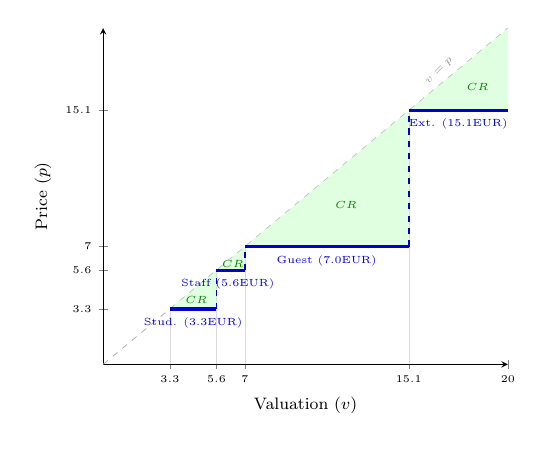
\begin{tikzpicture}[scale=0.75]
    \begin{axis}[
        xlabel={\footnotesize Valuation ($v$)}, ylabel={\footnotesize Price ($p$)},
        xmin=0, xmax=20, ymin=0, ymax=20,
        axis lines=left, xtick={3.3, 5.6, 7.0, 15.1, 20}, ytick={3.3, 5.6, 7.0, 15.1},
        tick label style={font=\tiny}, label style={font=\footnotesize}, clip=false
    ]
        \addplot[gray!60, thin, dashed, domain=0:20] {x}; 
        \node[gray!80, rotate=45, anchor=south] at (axis cs:17,17) {\tiny $v=p$};
        
        % Manual lines to avoid expansion errors
        \draw[gray!30, very thin] (axis cs:3.3,0) -- (axis cs:3.3,3.3);
        \draw[gray!30, very thin] (axis cs:5.6,0) -- (axis cs:5.6,5.6);
        \draw[gray!30, very thin] (axis cs:7.0,0) -- (axis cs:7.0,7.0);
        \draw[gray!30, very thin] (axis cs:15.1,0) -- (axis cs:15.1,15.1);

        \fill[green!20, opacity=0.6] (axis cs:3.3,3.3) -- (axis cs:5.6,5.6) -- (axis cs:5.6,3.3) -- cycle;
        \fill[green!20, opacity=0.6] (axis cs:5.6,5.6) -- (axis cs:7.0,7.0) -- (axis cs:7.0,5.6) -- cycle;
        \fill[green!20, opacity=0.6] (axis cs:7.0,7.0) -- (axis cs:15.1,15.1) -- (axis cs:15.1,7.0) -- cycle;
        \fill[green!20, opacity=0.6] (axis cs:15.1,15.1) -- (axis cs:20,20) -- (axis cs:20,15.1) -- cycle;
        
        \draw[blue!80!black, ultra thick] (axis cs:3.3,3.3) -- (axis cs:5.6,3.3) node[midway, below, font=\tiny] {Stud. (3.3EUR)};
        \draw[blue!80!black, ultra thick] (axis cs:5.6,5.6) -- (axis cs:7.0,5.6) node[pos=0.4, below, font=\tiny] {Staff (5.6EUR)};
        \draw[blue!80!black, ultra thick] (axis cs:7.0,7.0) -- (axis cs:15.1,7.0) node[midway, below, font=\tiny] {Guest (7.0EUR)};
        \draw[blue!80!black, ultra thick] (axis cs:15.1,15.1) -- (axis cs:20,15.1) node[midway, below, font=\tiny] {Ext. (15.1EUR)};
        
        \draw[blue!80!black, thick, dashed] (axis cs:5.6,3.3) -- (axis cs:5.6,5.6);
        \draw[blue!80!black, thick, dashed] (axis cs:7.0,5.6) -- (axis cs:7.0,7.0);
        \draw[blue!80!black, thick, dashed] (axis cs:15.1,7.0) -- (axis cs:15.1,15.1);
        
        \node[text=green!50!black] at (axis cs:4.6,3.8) {\tiny $CR$};
        \node[text=green!50!black] at (axis cs:6.4,6.0) {\tiny $CR$};
        \node[text=green!50!black] at (axis cs:12.0,9.5) {\tiny $CR$};
        \node[text=green!50!black] at (axis cs:18.5,16.5) {\tiny $CR$};
    \end{axis}
\end{tikzpicture}
\caption{Visualisation of Zeno's Partition: Consumer Rent ($CR$) within Mensa Pricing Intervals}
\label{fig:pricing_intervals}
\end{figure}

Although the university canteen example fits the Ali, Lewis and Vasserman model remarkably well, two distinctions must be noted for a comprehensive analysis:
In the benchmark (uniform price), students with a valuation of approximately between 3.3 and 5.6 are priced out because $v < p^* =6.13$. However, by disclosing their ID, students and staff can secure the rent shown in \cref{fig:pricing_intervals} and in \cref{tab:pricing_structure}, which represents a Pareto improvement compared to the zero surplus they would otherwise receive. Compared to the benchmark, the total consumer surplus increases under this tiered system because the 'external' and 'guest' types still retain significant surplus, while lower-valuation types (students) are finally able to enter the market.

This finding supports the paper's conclusion that consumer control over data, specifically the ability to share partial "rich" evidence, is a powerful tool for improving consumer welfare.

\subsection{Welfare Implications: Efficiency and Strategic Subsidy Targeting}
While the theoretical model focuses on profit, the real-world \textit{Mensa} uses this partition to manage heavy subsidies (EUR 21.56m in 2024).
Although the average price (EUR 7.75) is higher than the average revenue (EUR 6.13) in reality, the difference is almost exactly accounted for by state grants and social contributions.
The tiered disclosure system ensures that these state and social funds are effectively target toward the student and staff segments who would otherwise be priced out by guest/external pricing levels. This demonstrates that the "Mensa"  essentially acts as a social monopolist, using the 'rich evidence' of a student ID to distribute subsidies specifically to the lowest-valuation tiers.


\end{document}